\section{Convolutional Neural Networks}

\subsection{Architecture Overview}

在图像处理的任务中，图片的特征具有局部性，而全连接的传统神经网络引入了太多冗余的参数，既浪费又难以训练。因此，CNN 被提出以解决这个问题。CNN 的架构和传统神经网络架构类似，都具有输入层、隐藏层和输出层。不同的是，CNN 中每一层都是 $3$ 维的神经元，如下图所示：

\begin{figure}[H]
    \centering
    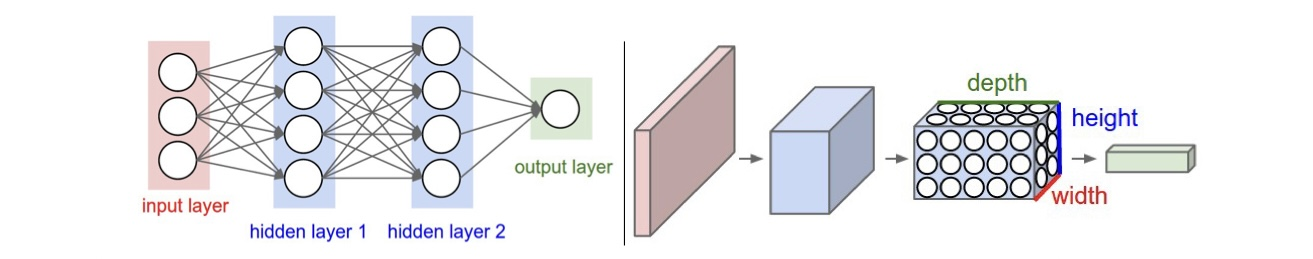
\includegraphics[width=0.8\linewidth]{figs/chapter4/conv.jpg}
\end{figure}

例如，CIFAR-10 数据集的输入可以是 $32\times32\times3$ 的，即 $\text{RGB}$ 三个通道分别有 $32\times32$ 的像素；其输出可以是 $1\times1\times10$，分别表示 $10$ 个分类上的得分。

下面来详细分析 CNN 中各种层的结构。

\subsection{Layers used to build CNN}

CNN 中主要有三种层：\textbf{Convolutinal Layer, Pooling Layer, Fully-Connected Layer}，将它们堆叠在一起就可以形成一个 CNN 的架构。

例如，[INPUT - CONV - RELU - POLL - FC] 就是一种简单的 CNN 架构。其中，CONV / FC 层具有需要学习的参数，而 RELU / POOL 层是固定的函数；CONV / FC / POOL 层都有超参数，而 RELU 没有。

\begin{figure}[H]
    \centering
    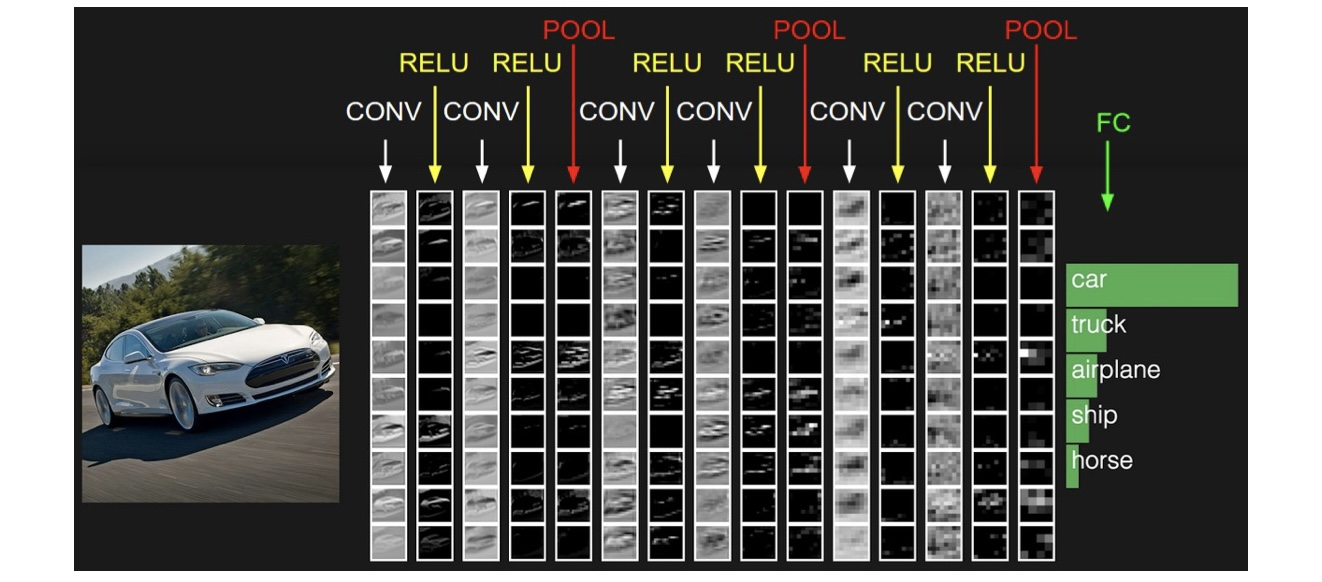
\includegraphics[width=0.8\linewidth]{figs/chapter4/layers.jpg}
\end{figure}

\paragraph{Convolutional Layer}

Convolutional Layer 是 CNN 的核心。其基本思想很简单，就是用一个\textbf{卷积核}（\textbf{filter} / \textbf{kernel}）在输入图像上扫一遍，得到输出图像，其中卷积核的参数就是神经网络要学习的参数。设输入深度为 $D_1$，则这个卷积核的深度也是 $D_1$，即将输入图像某一区域\textbf{所有层}的数据一起做线性组合；如果输入的深度是 $D_2$，那么我们需要 $D_2$ 个不同的卷积核，形成输出的不同层。

\begin{figure}[H]
    \centering
    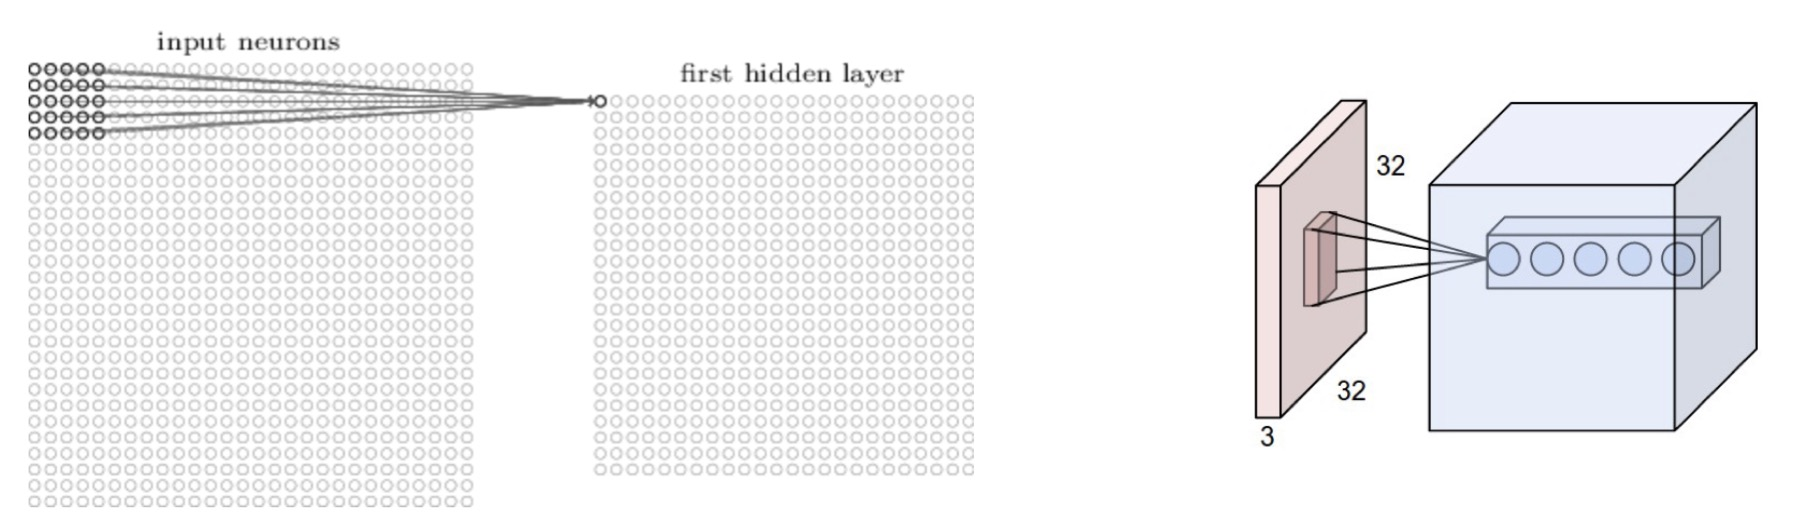
\includegraphics[width=1\linewidth]{figs/chapter4/filter.jpg}
\end{figure}

正式地说，设输入是一个 $W_1\times H_1\times D_1$ 的 $3$ 维数组（即上一层），Convolutional Layer 有以下几个超参数：

\begin{itemize}
    \item $K$：filters 的个数
    \item $F$：filters 的边长
    \item $S$：filters 进行扫描时的步长
    \item $P$：zero padding，在输入图像的边缘补充的长度

\end{itemize}
输出一个 $W_2\times H_2\times D_2$ 的 $3$ 维数组，其中：
\begin{align*}
W_2&=(W_1-F+2P)/S+1\\
H_2&=(H_1-F+2P)/S+1\\
D_2&=K
\end{align*}
在进行卷积操作时，我们需要注意计算得到的 $W_2$ 和 $H_2$ 是不是整数，如果不是，需要调整 $P$ 或者 $S$。另外，注意对于输出的每一个 depth slice，其上的神经元是由同一个卷积核算出来的，分享了同样的参数，这有助于减少 CNN 的参数数量。

\textbf{im2col} 是实现卷积操作的一个方法，正如其名 image to column，它将二维图像变成一个列向量以方便地实施卷积操作。举例说明，假设输入图像是 $[227\times227\times3]$，使用 $[11\times11\times3]$ 的卷积核并取步长为 $4$，想要得到 $[55\times 55\times96]$ 的输出。那么，我们将 $[11\times 11\times 3]$ 的卷积核拉伸成 $11\times11\times3=363$ 维的\textbf{行向量}，各卷积核拼接起来得到 $[96\times 363]$ 的参数矩阵；然后把输入图像中对应 $55\times 55$ 个位置的 $[11\times11\times3]$ 全拿出来拉伸成\textbf{列向量}并顺次拼接成 $[363\times 3025]$ 的矩阵；二者相乘即可得到 $[96\times 3025]$ 的矩阵，每一行的列向量还原成 $[55\times 55]$ 即得到输出结果。

\paragraph{Pooling Layer}

插入 Pooling Layer 是为了减小当前层的大小，与 Convolutional Layer 类似，它用一个 filter 扫描整个图像，然后做某种无参数的计算，如取 $\max$ (\emph{max pooling}) 或者 $\text{L2 norm}$ (\emph{L2-norm pooling}) 或者平均值 (\emph{average pooling}).

\begin{figure}[H]
    \centering
    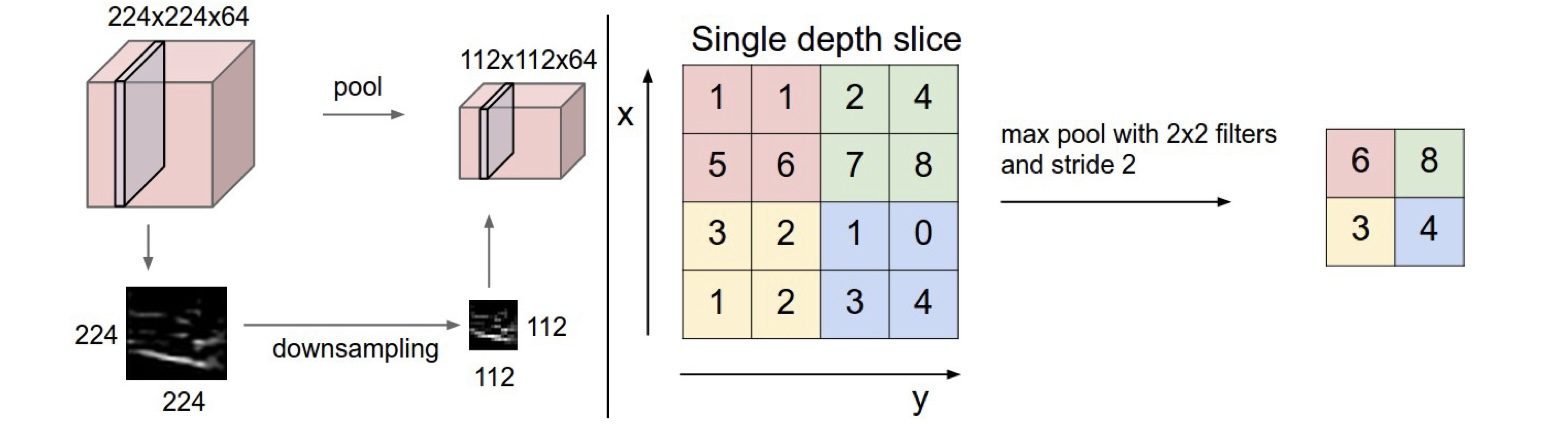
\includegraphics[width=0.8\linewidth]{figs/chapter4/pool.jpg}
\end{figure}

\paragraph{Fully-connected Layer}

CNN 中的全连接层和传统神经网络的全连接层一模一样，一般最后连接输出层的时候用全连接层。

FC Layer 可以和 Conv Layer 相互转化：

\begin{itemize}
    \item Conv 转 FC：只需要强行设定 FC 中某些权重为 $0$；
    \item FC 转 Conv：设定 Conv 卷积核大小与输入相同，那么一次卷积运算相当于 FC 前一层到后一层的某一个神经元的运算。
\end{itemize}


\subsection{CNN Architectures}

上一节讲了 CNN 中主要的三种层，这一节讲如何把它们的组合在一起形成 CNN.

\paragraph{Layer Patterns}

最常见的各种层的组合是：
\[
\texttt{INPUT} \to [[\texttt{CONV}\to\texttt{RELU}] \times N \to \texttt{POOL} ] \times M \to [\texttt{FC}\to\texttt{RELU}]\times K \to\texttt{FC}
\]
即若干 CONV-RELU layers，选择性地接 POOL layer，重复该结构直到最后接上传统的神经网络。

实践中注意一点：相比用一个具有较大卷积核的卷积层，更好的是使用多个具有较小卷积核的卷积层堆叠起来，因为一方面，堆叠起来的层引入更多非线性因素，使神经网络更强大；另一方面，后者具有更少的参数。

\paragraph{Layer Sizing Patterns}

\begin{itemize}
    \item \textbf{input layer}：最好能被 $2$ 整除很多次；
    \item \textbf{conv layers}：应使用小的 filters（如 $3\times 3$ 或最多 $5\times 5$），使用步长 $S=1$，并且使用 zero padding 保证输出图像的大小和输入的大小相等（取 $P=(F-1)/2$ 即可），这样能够防止略过图像边缘的信息，而把缩小 feature map 的任务交给 Pooling layer；
    \item \textbf{pool layers}：负责缩小输入的大小。最常用一个 $2\times 2$ 的 filter 以步长为 $2$ 扫描一遍，丢掉恰好 $75\%$ 的结果；也可以使用 $3\times 3$ 的 filter，但是基本不用 $>3$ 的 filter，因为这样太过 aggresive 而使得结果变差。

\end{itemize}
\paragraph{Case studies}

有一些经典的 CNN 结构有一个名字，例如：

\begin{itemize}
    \item \href{http://yann.lecun.com/exdb/publis/pdf/lecun-98.pdf}{\textbf{LeNet}}：由 Yann LeCun 在 1990's 实现。
    \item \href{https://proceedings.neurips.cc/paper/2012/file/c399862d3b9d6b76c8436e924a68c45b-Paper.pdf}{\textbf{AlexNet}}：由 Alex Krizhevsky, Ilya Sutskever 和 Geoff Hinton 实现，在 2012 年 ImageNet ILSVRC 比赛中以绝对优势夺冠，并使得 CNN 从此广受欢迎。
    \item \href{https://arxiv.org/abs/1311.2901}{\textbf{ZF Net}}：由 Matthew Zeiler 和 Rob Fergus 实现，在 ILSVRC 2013 夺冠。
    \item \href{https://arxiv.org/abs/1409.4842}{\textbf{GoogLeNet}}：由 Szeged 等人实现，在 ILSVRC 2014 夺冠。
    \item \href{https://arxiv.org/abs/1409.1556}{\textbf{VGGNet}}：由 Karen Simonyan 和 Andrew Zisserman 实现，是 ILSVRC 2014 的第二名。
    \item \href{https://arxiv.org/abs/1512.03385}{\textbf{ResNet}}：由何恺明等人实现，在 ILSVRC 2015 夺冠。

\end{itemize}
